% ! Author = Omar Iskandarani
% ! Title  = Reaction to Han et al. (2025): Attosecond Chiral Photoionization in the Swirl--String Theory Framework
% ! Date   = Sept 3, 2025
% ! Affiliation = Independent Researcher, Groningen, The Netherlands
% ! License = © 2025 Omar Iskandarani. All rights reserved.

\documentclass[smallextended]{svjour3}       % One-column layout
%\documentclass[twocolumn]{svjour3}          % Uncomment for two-column layout
\smartqed  % flush right qed marks
\usepackage{cite}
\usepackage{float}

%========================================================================================
% PACKAGES AND DOCUMENT CONFIGURATION
%========================================================================================

% ===== Tikz =====
\usepackage{tikz}
\usepackage{pgfplots}
\pgfplotsset{compat=1.18}
\usetikzlibrary{arrows.meta,calc,decorations.markings,positioning}
\usetikzlibrary{fpu}

% Encoding & language
\usepackage[utf8]{inputenc}
\usepackage[T1]{fontenc}
\usepackage[english]{babel}

% Layout & typography
\usepackage{lmodern} % Use scalable Latin Modern fonts
\usepackage[margin=2.2cm]{geometry}
\usepackage{microtype}

% Math & symbols
\usepackage{amsmath,amssymb,amsfonts,bm}

% Tables
\usepackage{booktabs}

% Units & numbers
\usepackage{siunitx}
\sisetup{detect-all=true,range-phrase = --,range-units = single}
% Define Å as an SI unit for convenience
\DeclareSIUnit\angstrom{\text{\AA}}

% Quotes (for biblatex)
\usepackage{csquotes}

% Bibliography (BibLaTeX + biber)
\usepackage[backend=biber,style=numeric,sorting=none,doi=true,url=false,maxbibnames=99]{biblatex}
\addbibresource{refs.bib}

% Hyperlinks
\usepackage[colorlinks=true,linkcolor=blue,citecolor=blue,urlcolor=blue]{hyperref}

% ==== Macros for SST ====
\newcommand{\vswirl}{\mathbf{v}_{\!\boldsymbol{\circlearrowleft}}}
\newcommand{\vswirlcw}{\mathbf{v}_{\!\boldsymbol{\circlearrowright}}}
\newcommand{\SwirlClock}{S_t^{\boldsymbol{\circlearrowleft}}}
\newcommand{\SwirlClockcw}{S_t^{\boldsymbol{\circlearrowright}}}
\newcommand{\vnorm}{\lVert \mathbf{v}_{\!\boldsymbol{\circlearrowleft}}\rVert}
\newcommand{\rhoF}{\rho_{\!f}}


\sisetup{detect-all=true,range-phrase = --,range-units = single}
% Define Å as an SI unit for convenience
\DeclareSIUnit\angstrom{\text{\AA}}


% ---- Local bibliography (self-contained build) ----
\begin{filecontents*}{refs.bib}
@article{Han2025,
  author  = {Han, M. and Ji, J.-B. and Blech, A. and Goetz, R. E. and Allison, C. and Greenman, L. and Koch, C. P. and W\"orner, H. J.},
  title   = {Attosecond control and measurement of chiral photoionization dynamics},
  journal = {Nature},
  year    = {2025},
  doi     = {10.1038/s41586-025-09455-4},
  note    = {online 27 Aug 2025}
}
\end{filecontents*}


\title{Chirality as Time Asymmetry: A Swirl--String Theory Interpretation of Attosecond Photoionization Delays}
\author{Omar Iskandarani\\\small Independent Researcher, Groningen, The Netherlands}
\date{September 3, 2025}


\begin{document}
\maketitle


\begin{abstract}
Recent attosecond-resolved photoionization measurements by Han et al.~(\emph{Nature}, 2025) reveal enantiomer-dependent time delays up to \SI{240}{\atto\second} in methyloxirane. We interpret these findings within the Swirl--String Theory (SST) framework, where chirality is modeled as a local time-asymmetric property associated with orientation-dependent circulation fields. We show that observed delays cannot be attributed to relativistic time dilation, but are consistent with anisotropic scattering along foliation leaves in the swirl field. Delay magnitudes correspond to \AA-scale path differences, suggesting direct measurable influence of Swirl Clock asymmetry on continuum electron dynamics. SST predicts that time-asymmetric effects should also arise in topologically asymmetric systems beyond molecular chirality.
\end{abstract}



\section{Introduction}
Chirality plays a central role in chemistry, biology, and physics, yet its connection to the arrow of time remains elusive. Recent experimental advances in attosecond science have enabled time-resolved measurements of photoionization in chiral molecules. Notably, Han et al.~\cite{Han2025} reported enantiomer-dependent attosecond delays in methyloxirane, prompting new questions about the temporal structure of chiral interactions.


In this work, we explore these findings through the lens of Swirl--String Theory (SST), a topological hydrodynamic model in which particles are modeled as quantized circulation knots in a universal swirl medium. A key construct in SST is the \emph{Swirl Clock}, a local directional time rate determined by the orientation and magnitude of swirl velocity. Within this framework, chirality manifests not only geometrically but dynamically---as a time-asymmetric property with measurable consequences.


\section{Summary of Han et al. (2025)}
Han et al.~\cite{Han2025} performed attosecond-resolved photoelectron spectroscopy using circularly polarized extreme-ultraviolet pulse trains with an infrared probe (RABBIT) to ionize gas-phase methyloxirane. Key results include:


\begin{itemize}
    \item \textbf{Chiral delay:} Forward--backward photoemission delays of approximately \SI{60}{\atto\second}, reversing with enantiomer.
    \item \textbf{Angular delay spread:} Angle-resolved delays up to \SI{240}{\atto\second}.
    \item \textbf{Continuum chirality:} Additional \SI{60}{\atto\second} delay in continuum--continuum transitions, persisting post-ionization.
\end{itemize}


These delay asymmetries suggest a directional time structure embedded in the chiral photoionization process.


\section{Swirl--String Theory and the Swirl Clock}
SST posits that spacetime contains an underlying swirl medium supporting quantized circulation loops, interpreted as elementary particles. Each localized swirl excitation possesses a swirl velocity field $\vswirl$, with associated circulation and helicity. Proper time within the swirl is modulated by the swirl speed $\vnorm$ as:


\begin{equation}
  dt_{\text{local}} = dt_{\infty}\,\sqrt{1 - \frac{\vnorm^2}{c^2}}.
\end{equation}


The Swirl Clock $\SwirlClock$ refers to this direction-sensitive local rate. In chiral molecules, opposite enantiomers correspond to reversed Swirl Clock orientations ($\SwirlClock$ vs.~$\SwirlClockcw$). As a result, time asymmetries can emerge in electron emission depending on swirl orientation.

% Pure TikZ graphical abstract for SST chiral delays
% Drop this figure into your LaTeX document. Ensure in preamble:
%   \usepackage{tikz}
%   % (optional) libraries if you extend styles:
%   % \usetikzlibrary{arrows.meta,calc,decorations.markings,positioning}
% Requires siunitx already loaded (present in your paper).


\begin{figure}[t]
  \centering
  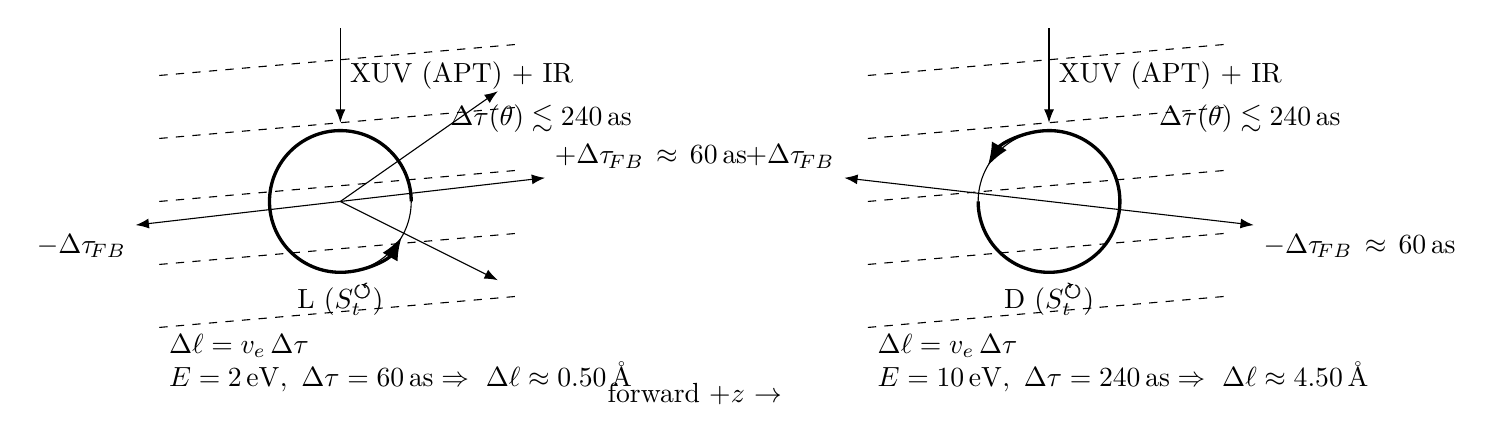
\begin{tikzpicture}[x=1cm,y=1cm,>=Latex]
    % ----- left panel: L enantiomer (ccw Swirl Clock) -----
    \begin{scope}[shift={(0,0)}]
      % foliation leaves (schematic, dashed planes)
      \foreach \y in {-1.6,-0.8,0,0.8,1.6} \draw[dashed] (-2.3,\y) -- (2.3,\y+0.4);
      % molecule + swirl (ccw)
      \draw (0,0) circle (0.9);
      \draw[very thick,->] (0.9,0) arc[start angle=0,end angle=330,radius=0.9];
      \node at (0,-1.25) {L ($\SwirlClock$)};
      % XUV+IR excitation
      \draw[->] (0,2.2) -- (0,1.0) node[midway,right] {XUV (APT) + IR};
      % forward/back emission with sign of FB delay
      \draw[->] (0,0) -- (2.6,0.3) node[above right] {$+\Delta\tau_{\!FB}\,\approx\,\SI{60}{as}$};
      \draw[->] (0,0) -- (-2.6,-0.3) node[below left] {$-\Delta\tau_{\!FB}$};
      % angular spread annotation
      \draw[->] (0,0) -- (2.0,1.4);
      \draw[->] (0,0) -- (2.0,-1.0);
      \node[align=left] at (2.55,1.05) {$\Delta\tau(\theta)\lesssim\SI{240}{as}$};
      % path-difference mapping callout
      \node[align=left,anchor=west] at (-2.3,-2.05) {$\Delta\ell=v_e\,\Delta\tau$\\$E=\SI{2}{eV},\ \Delta\tau=\SI{60}{as}\Rightarrow\ \Delta\ell\approx\SI{0.50}{\angstrom}$};
    \end{scope}


    % ----- right panel: D enantiomer (cw Swirl Clock) -----
    \begin{scope}[shift={(9,0)}]
      % foliation leaves
      \foreach \y in {-1.6,-0.8,0,0.8,1.6} \draw[dashed] (-2.3,\y) -- (2.3,\y+0.4);
      % molecule + swirl (cw)
      \draw (0,0) circle (0.9);
      \draw[very thick,->] (-0.9,0) arc[start angle=180,end angle=510,radius=0.9];
      \node at (0,-1.25) {D ($\SwirlClockcw$)};
      % XUV+IR excitation
      \draw[->] (0,2.2) -- (0,1.0) node[midway,right] {XUV (APT) + IR};
      % forward/back emission with opposite sign
      \draw[->] (0,0) -- (2.6,-0.3) node[below right] {$-\Delta\tau_{\!FB}\,\approx\,\SI{60}{as}$};
      \draw[->] (0,0) -- (-2.6,0.3) node[above left] {$+\Delta\tau_{\!FB}$};
      % angular spread annotation
      \node[align=left] at (2.55,1.05) {$\Delta\tau(\theta)\lesssim\SI{240}{as}$};
      % path mapping at higher energy
      \node[align=left,anchor=west] at (-2.3,-2.05) {$\Delta\ell=v_e\,\Delta\tau$\\$E=\SI{10}{eV},\ \Delta\tau=\SI{240}{as}\Rightarrow\ \Delta\ell\approx\SI{4.50}{\angstrom}$};
    \end{scope}


    % global axis hint
    \node at (4.5,-2.45) {forward $+z$ $\rightarrow$};
  \end{tikzpicture}
  \caption{Swirl Clock--induced chiral photoionization delays (TikZ schematic). Left: L enantiomer ($\SwirlClock$) with $+\Delta\tau_{\!FB}$; Right: D enantiomer ($\SwirlClockcw$) with $-\Delta\tau_{\!FB}$. Dashed lines suggest foliation leaves guiding anisotropic swirl scattering; labels show delay-to-path mapping examples.}
  \label{fig:tikz-sst-chiral-delays}
\end{figure}



\section{Delay Analysis and Path Mapping}
For $\vnorm = \SI{1.094e6}{\meter\per\second}$ (canonical swirl speed), time dilation is negligible: for a RABBIT $2\omega$ period $T = \SI{1.33}{\femto\second}$, the resulting shift is
\begin{equation}
  \Delta t_{\text{dil}} \approx T\!\left(1 - \sqrt{1 - \left(\tfrac{\vnorm}{c}\right)^2}\right) \approx \SI{8.85e-3}{\atto\second},
\end{equation}
which is three orders of magnitude below observed delays. Instead, we associate the attosecond delays with effective path differences
\begin{equation}
  \Delta \ell = v_e\,\Delta \tau, \qquad v_e(E) = \sqrt{\tfrac{2E}{m_e}},
\end{equation}
where $v_e$ is the electron velocity for kinetic energy $E$, and $\Delta \tau$ is the measured delay.


\begin{table}[h]
  \centering
  \caption{Delay-to-path mapping.}
  \begin{tabular}{@{}ccc@{}}
    \toprule
    $E$ (eV) & $\Delta \tau$ (as) & $\Delta \ell$ (\AA) \\
    \midrule
    2  & 60  & 0.50 \\
    5  & 120 & 1.59 \\
    10 & 240 & 4.50 \\
    \bottomrule
  \end{tabular}
\end{table}



    \begin{figure}[t]
    \centering
    \begin{tikzpicture}
    \begin{axis}[
    width=0.82\linewidth, height=0.48\linewidth,
    xlabel={Electron kinetic energy $E$ (eV)},
    ylabel={Path difference $\Delta\ell$ (\AA)},
    xmin=2, xmax=12,
    ymin=0, ymax=5.1,
    grid=both,
    legend cell align=left,
    legend pos=north west,
    tick label style={/pgf/number format/fixed},
    % scaled y ticks=false, % uncomment if you don't want scientific notation
    ]

    %---- enable high-precision arithmetic for constant evaluation ----
    \pgfkeys{/pgf/fpu=true}
    \pgfmathsetmacro{\me}{9.1093837015e-31}   % kg
    \pgfmathsetmacro{\eVJ}{1.602176634e-19}   % J
    % Precompute K = 1e10 * sqrt(2*eVJ/me), so Δℓ(Å) = K * Δτ(s) * sqrt(E/eV)
    \pgfmathsetmacro{\KAng}{1.0e10 * sqrt(2*\eVJ/\me)}
    \pgfmathsetmacro{\tauA}{60e-18}           % s
    \pgfmathsetmacro{\tauB}{240e-18}          % s
    \pgfkeys{/pgf/fpu=false}

    %---- numerically stable function: Δℓ(Å) = K * τ * sqrt(E) ----
    \pgfmathdeclarefunction{dAng}{2}{%
        \pgfmathparse{\KAng*(#2)*sqrt(#1)}%
    }

    %---- curves ----
    \addplot+[smooth, thick, domain=2:12, samples=300] { dAng(x, \tauA) };
    \addlegendentry{$\Delta\tau = 60~\mathrm{as}$}

    \addplot+[smooth, thick, domain=2:12, samples=300] { dAng(x, \tauB) };
    \addlegendentry{$\Delta\tau = 240~\mathrm{as}$}

    %---- annotated markers ----
    \pgfmathsetmacro{\dAatTwo}{\KAng*\tauA*sqrt(2)}
    \pgfmathsetmacro{\dBatTen}{\KAng*\tauB*sqrt(10)}

    \addplot+[only marks, mark=x, mark size=2pt] coordinates {(2,\dAatTwo)};
    \node[anchor=south west, font=\scriptsize]
    at (axis cs:2,\dAatTwo)
        {~$2~\mathrm{eV}\ \to\ \pgfmathprintnumber[fixed,precision=2]{\dAatTwo}\ \text{\AA}$};

    \addplot+[only marks, mark=x, mark size=2pt] coordinates {(10,\dBatTen)};
    \node[anchor=south west, font=\scriptsize]
    at (axis cs:10,\dBatTen)
        {~$10~\mathrm{eV}\ \to\ \pgfmathprintnumber[fixed,precision=2]{\dBatTen}\ \text{\AA}$};

    \end{axis}
    \end{tikzpicture}
    \caption{Å–scale path difference $\Delta\ell=v_e(E)\,\Delta\tau$ for $\Delta\tau\in\{60,240\}$ as over $E\in[2,12]$ eV.}
    \label{fig:tikz_pathdiffs}
    \end{figure}

These path differences align with \AA-scale structural asymmetries, supporting a geometric--dynamical interpretation of chirality.


\section{Interpretation in SST}
Within SST, the observed delays arise naturally from anisotropic swirl scattering:
\begin{itemize}
    \item \textbf{Chiral delay:} Reversal of Swirl Clock orientation leads to reversed forward--backward time asymmetry.
    \item \textbf{Angular dispersion:} Variation in the swirl potential across emission directions induces delay spread.
    \item \textbf{Continuum propagation:} Persistence of asymmetry in the free-electron phase implies Swirl Clock memory beyond ionization.
\end{itemize}
This distinguishes SST from models where chirality is purely geometrical and lacks dynamical time asymmetry.


\section{Discussion}
SST provides a physically consistent mechanism for time-asymmetric effects without relying on relativistic corrections. The model predicts similar Swirl Clock--induced asymmetries in systems lacking conventional chirality but exhibiting topological asymmetry (e.g., molecular knots or asymmetric confinement fields). Future ultrafast experiments could probe such systems for attosecond-scale delays to test the generality of swirl-based time asymmetry.


\section{Conclusion}
Han et al.'s results can be interpreted as experimental evidence for dynamic chirality rooted in directional time evolution. The Swirl--String framework offers a predictive and falsifiable model that links topology, geometry, and proper time in a unified picture. The correspondence between observed delays and predicted path asymmetries suggests that chirality is not merely a spatial property---but a temporal one.


\printbibliography


\end{document}

